\section{Reputation}
\subsection{What is Reputation?}
blabla text here ... score associated to an account... cannot be transferred... used as voting weight... hoepfully leading to meritocratic decision making.
FIXME FIXME

There are many reputation scores per user ... local to domains or skills.... not one global score. Also Reputation decays with time.



Reputation earned in Colony will primarily be earned from completing tasks, and the amount of reputation earned will be based on a combination of the performance of the user completing the task, and the payout associated with the task itself.

We note this creates a problem we have affectionately taken to calling the ‘Palo Alto Problem’, whereby users who are paid more for the same work - such as those living in Palo Alto may be compared to those in South America - earn more influence in the colony. While we would like to solve this problem, we have been unable to do so to date; any possible solution either seems to introduce a great deal of complexity to the system or provide the ability for a bad actor to accrue undue influence in the colony.
\subsubsection{Reputation per Domain}
Users have reputation local to any domain. Earning rep in a domain earns you rep in any parent domain. Losing rep also affects all children.
Top Level reputation ...

beyond this we also want skill tags:

\subsubsection{Skill hierarchy}

The existence of domains that form the organisational hierarchy of a colony was described in section \ref{sec:domains}. In addition to this organisational hierarchy (which is unique to each colony), the Colony Network also maintains a hierarchy of skill domains (or just `skills'), which is available for all colonies to use. A user's good or bad activity associated with either of these hierarchies will earn or lose them the corresponding reputation, though only in a single colony.\footnote{It is hopefully clear that allowing users to earn reputation in one colony and then use it to influence decisions in another would be ripe for abuse.}

For example, when a task is created, as well as being placed in a particular domain in the colony, it is also tagged with a skill from the skill hierarchy. When the worker earns reputation for succesfully completing the task, they will earn reputation in all the relevant domains and skills. Conversely, if they are to lose reputation because their work is found inadequate, they will do so in all the relevant domains ad skills.

\subsection{Earning reputation}
The only way that reputation is created in a colony is when it is FIXME

\subsubsection{Bootstrapping reputation}

Since a large portion of a colony's decision making procedure rests on reputation weighted voting, we are presented with a bootstrapping problem for new colonies.
When a colony is new, no-one has yet completed any work in it and so nobody will have earned any reputation. Consequently,no dospites could be resolved as no-one would be able to vote on them. \\
Therefore, when a colony is created, the creator can nominate addresses to have initial reputation assigned to them to allow the colony to bootstrap itself. There will be a global limit on the reputation that can be assigned in this manner in order to prevent an extreme reputation aristocracy. Given that reputation decays over time, this initial bootstrapping of reputation will not have an impact on the long-term operation of the colony. \textbf{This is the only time that reputation can be created without associated work being done.}

At first glance it may appear as if the same bootstrapping problem presents itself whenever a domain is created - if the domain has had no work done in it, then who has the authority to make decisions? We do not wish to allow the creation new reputation here, as this would devalue reputation already earned in the colony by users completing work. Luckily we can proceed without any new reputation: we simply accept the fact the new domain has no reputation in it. The colony is still able to make decisions and resolve disputes, because any objections can be escalated to a parent domain if necessary. Furthermore, even this escalation is not necessarily required in the event of a disagreement, because, even if there is no reputation in the domain to contribute to the decision, users will still be able to vote based on their reputation in relevant skills.

\subsubsection{Earning Reputation by contributing to a task}
admin, worker, evaluator.... FIXME

\subsubsection{Earning Reputation as a result of Disputes}
see title.



\subsection{Losing Reputation}

\subsubsection{Reputation Decay}
All reputation decays over time.\\
Every 600000 blocks, a user’s reputation in any domain or skill decays by a factor of 2. This decay occurs continuously, rather than being a step change every three months to ensure there are as few incentives to earn reputation at any particular time.

\subsubsection{Losing Reputation due to a Negative Evaluation}
working on a task. bad review. lose rep....


\subsubsection{Losing Reputation due to Bad Behaviour}
disputes and how they affect rep....


Whenever a user stakes tokens, they are also risking their reputation. If the tokens are lost, then they also lose reputation. Reputation is not staked, and so while at risk it can still be used by users to vote on decisions where that reputation is relevant - they only lose the voting power associated with the reputation once it is lost. However, it should be noted that the same is not true of colony tokens - once staked, their voting power is lost. However, we expect that users will only ever stake a small proportion of their tokens - only small amounts of tokens are staked in the Colony Network to ensure a tangible financial punishment to the staking user can be made if they are a badly behaving actor.

The amount of tokens to be staked and reputation that can be lost depend on the context of the action being taken. The greater the proportion of reputation in the colony that is potentially inconvenienced by the action being taken in the event that it is fraudulent, the greater the reputation and tokens that must be staked by the user to take the action.




\newcommand{\rc}{root colony\ }
\newcommand{\rct}{root colony token\ }
\newcommand{\rcts}{root colony tokens\ }
\newcommand{\rcth}{root colony token holder\ }
\newcommand{\rcths}{root colony token holders\ }

\section{Calculating Reputation: Miners \& Merkle Proofs}\label{sec:reputationmining}
We see that the reputation system is a core component of the decentralised colony network. By carefully balancing the rewards and penalties we aim to keep every users' incentives aligend with the colony and the colony network. Since reputation can only be \emph{earned} and not bought, the system fosters a more meritocratic from of decision making than pure token-weighted voting can hope to achieve. The continuous decay of reputation ensures that the influece conveyed by reputation is recent and up-to-date; it prevents a reputation aristocracy and allows for a fluid passing of control from one set of contributors to another over time.\\
How well the parameters of the reputation system balance out competing interests will have to be subject to empirical review when the colony network begins live operation and any parameters proposed in this document should be seen as suggestions, not prescriptions for the final network.\\
Due to the combined complexity of reputation scores across multiple colonies, domains, skills; growing due to tasks completed and disputes won; shrinking due to decay and poor performance; \textbf{reputation scores cannot be stored and calculated on-chain}. Instead, the calculations will all take place off-chain, the results of which will be reported to the blockchain by participating \rcths -- in a process resembling a proof-of-stake blockchain consensus protocol. We call this procedure \textbf{``Reputation Mining''}.\\
The calculation whose result the miners are submitting, is determined by the activites that have taken place in the colonies and can be fully deterministically derived from the ethereum blockchain. Game-theoretically the system is protected similary to the off-chain calculations of truebit and golem??? (REFREFREFERENCE) in the \emph{while the calculation cannot be done on-chain, an incorrect calculation can always be proved to be wrong.}


\subsection{The Reputation Tree and the ReputationRootHash}
A reputation consists of the following data:
$$
R = 
\begin{cases}
 id & \textnormal{the id of a skill or domain identifying the type of reputation},\\
 colony\_id & \textnormal{the colony the reputation is held in},\\
 user & \textnormal{the address holding the skill},\\
 amount & \textnormal{the numerical value of the reputation}.
\end{cases}
$$
All individual reputations are assembled into the \textbf{``Reputation Tree''} which is a merkle tree of all individual reputations in a colony and the cumulative totals. (Note: with the \ascode{user} is set to zero, the corresponding amount is taken to represent the total of all such reputation held by users in this colony.)\\
All reputations held by all users in all colonies are ordered in a list. The elements of this list are hashes pairwise, to end up with a shorter list of hashes. This process is repeated until only one hash remains: the \ascode{ReputationRootHash}, $\mathcal{H}$.
\begin{center}
\begin{tikzpicture}
 \node at (0,-5) (r1) {$R_1$};
 \node at (1.5,-5) (r2) {$R_2$};
 \node at (3,-5) (r3) {$R_3$};
 \node at (4.5,-5) (r4) {$R_4$};
 \node at (6,-5) (rdots) {$\cdots$};
 \node at (8,-5) (rn) {$R_n$};
 %
 \node at (0,-4) (r1hash) {$\mathcal{H}(R_1)$}
  edge[-] (r1);
 \node at (1.5,-4) (r2hash) {$\mathcal{H}(R_2)$}
  edge[-] (r2);
 \node at (3,-4) (r3hash) {$\mathcal{H}(R_3)$}
  edge[-] (r3);
 \node at (4.5,-4) (r4hash) {$\mathcal{H}(R_4)$}
  edge[-] (r4);
 \node at (8,-4) (rnhash) {$\mathcal{H}(R_n)$}
  edge[-] (rn);
 %
 \node at (1,-2.5) (r12) {$\mathcal{H}_{1,2}$}
  edge[-] (r1hash)
  edge[-] (r2hash);
 \node at (3.75,-2.5) (r34) {$\mathcal{H}_{3,4}$}
  edge[-] (r3hash)
  edge[-] (r4hash);  
 \node at (7,-2.5) (rnn) {$\mathcal{H}_{n,n-1}$}
  edge[-] (rnhash)
  edge[dashed] (6.5,-4);
 %
 \node at (2.5,-1) (r14) {$\mathcal{H}_{12,34}$}
  edge[-] (r12)
  edge[-] (r34);
 %
 \node[draw, fill=gray!5] at (4,0) (root) {\texttt{ReputationRootHash}};
 \node[below = 1mm of root] (dummy) {\phantom{a}}
  (dummy.north west) edge[dashed] (r14)
  (dummy.north east) edge[dashed] (rnn);
 %
 %
 \node at (4,-6) (label) {\textnormal{The Reputation Tree}};
\end{tikzpicture}
\end{center}

In the event of a starting or an intermediate array being an odd number (which will always happen for a starting array that is not a power of two), the hash contained in the last element is hashed with itself.

The \ascode{ReputationRootHash} is the data we record on the blockchain. It represents an integrity check for the entire reputation system and whenever a user wishes to make use of their reputation, the can submit a merkle proof starting at the reputation they wish to make use of and ending at the \ascode{ReputationRootHash}.

\subsection{Calculating the new root hash}
The \rcth takes the last reputation state, and decays all reputation held by all users in all colonies, in the order of the leaves in the tree. They then take the set of reputation gains or losses due to good or bad behaviour that were not in the last state submitted, and are to be included in the next state. They apply the reputation updates to each user, in each colony, as is appropriate, to end up with a new list of reputations for all users and colonies. These new reputations are then hashed and assembled into a new merkle tree yielding an updated \ascode{ReputationRootHash}.

While the calculation is to large to be done on-chain due to technical (gas limit) and economic (gas cost) limitations, it is expected that this calculation can easily be performaed by any consumer grade laptop computer.

\subsection{Submission of a new root hash}
%
\subsubsection*{What is submitted?}
The final \ascode{ReputationRootHash} is submitted to the contract by the miner along with the number of leaves in the tree. Further, the miner also submits the IPFS/Swarm hash of a document containing the entire state tree (though this is only for convenience; any user can construct this locally based on the blockchain history).
%
\subsubsection*{Who can submit a new root hash?}
Since any user can calculate the correct root hash locally, it would be possible for \emph{any} \rcth to submit the hash to the contract.
It is however undesirable to have too many submissions for every update. We propose a mechanism that only allows some \rcths to submit results to begin with. To participate in the mining process, \rcths must stake some of their tokens to become `reputation miners'. A submission will only be accepted from a miner if \ascode{SHA3(address, N, hash, ... )} is sufficiently small.  At the beginning of the submission window, the target is set to 0 and slowly increases such that after 150 blocks all submissions are accepted\footnote{Some minimal \rct holding requirements may apply to ward off a denial of service attack with thousands of false submissions.}. Here N is some number greater than 0 and less than the number of tokens the \rcth address has staked, meaning that users with a large stake have a higher chance of qualifying to submit a hash than smaller stake holders.
%
\subsubsection*{Verifying a submission}
If only one state is submitted by the end of the submission period, then the new state is accepted, and proposals of the next state can begin to be made.  If more than one state has been submitted, then either someone has made a mistake, or there is a malicious entity trying to introduce a fraudulent reputation change. In this event, the a challenge protocol can establish which state is incorrect (see Section \ref{sec:challengeresponse})

\subsubsection*{Mining Rewards}

When a state is accepted, a small number of (newly generated) \rcts are made available for the user who first submitted the correct state to claim as a reward. When the user claims this payout, they receive a corresponding amount of reputation in the \rc (a special mining skill, which only users in the root colony can earn by performing this task). This reputation update is no different from any other, aside from the limitations of who is able to earn it, and will be included in a subsequent reputation update cycle.

\subsection{Dealing with false submissions}\label{sec:challengeresponse}
The challenge-response mechanism detailed below relies heavily on merkle proofs, so it will be useful to establish some notation.

\subsubsection{Merkle Proofs}
Consider the merkle tree shown in figure below. In order to prove that the element \ascode{A} is in the tree with root \ascode{G}, one submits a merkle proof containing the following information: \ascode{A, [B,F], [l,l]}. The first argument is the element whose existence is to be proved. The second argument is the list of hashes that \ascode{A} should be hashed pairwise with. The last argument is an array of \ascode{l}'s and \ascode{r}'s that indicates whether the next element in question should be hashed on the left or the right of the hash calculated so far. So to show that \ascode{C} was in the tree with root \ascode{G}, the proof would be of the form \ascode{C, [D,E], [l,r]}.
\begin{center}
 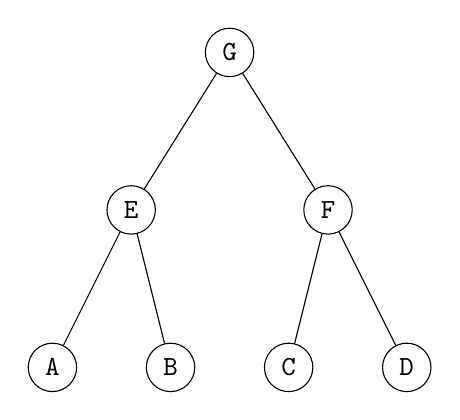
\begin{tikzpicture}
  \node[shape=circle, draw] at (0,-4) (a) {\texttt{A}};
  \node[shape=circle, draw] at (1.5,-4) (b) {\texttt{B}};
  \node[shape=circle, draw] at (3,-4) (c) {\texttt{C}};
  \node[shape=circle, draw] at (4.5,-4) (d) {\texttt{D}};
  %
  \node[shape=circle, draw] at (1,-2) (e) {\texttt{E}}
   edge[-] (a)
   edge[-] (b);
  \node[shape=circle, draw] at (3.5,-2) (f) {\texttt{F}}
   edge[-] (c)
   edge[-] (d);
  %
  \node[shape=circle, draw] at (2.25,0) (g) {\texttt{G}}
   edge[-] (e)
   edge[-] (f);
 \end{tikzpicture}
\end{center}
Note also that the array of \ascode{l}'s and \ascode{r}'s nothing more than a binary representation of the leaf node's index in the tree. When expressed in this way, we refer to the index as the `path' in the merkle proof. We refer to the objects that get hashed along the way (eg \ascode{[D,E]}) as the `siblings'.
%
\subsubsection{The Challenge-Response Protocol}
We assume that the correct hash is one of the  submitted hashes. This is a reasonable assumption, as only one \rcth out of all miners is required to make a submission, and there is an incentive for them to do so (\rc reputation). Thus our task is not to validate the correct hash but to invalidate the false ones.













